% Author : Alexandre Quenon
% Last update : July 5, 2014

% % % % % % %
%  Packages %
% % % % % % %

%---Base packages-
\documentclass[t]{beamer}			% document type
	% options are:
		% c or t to place the text at the vertical center or top of the slides
	% some packages are automatically loaded: 
		% amsmath, amsthm, amssymb; color, xcolor; hyperref
\usepackage[utf8]{inputenc}			% encoding
\usepackage[T1]{fontenc}			% accent
\usepackage{lmodern}				% latin font
\usepackage{wrapfig}
\usepackage{hyperref}
\hypersetup{
    colorlinks=true,
    urlcolor=cyan,
}
\usepackage{multicol}
\graphicspath{{figures/}}

%---Language(s)
\usepackage[english,frenchb]{babel}	% last language = typography by default
\addto\captionsfrench{				% to change the french names of...
	\renewcommand{\tablename}{\textsc{Tableau}}	% (default \textsc{Table})
}

%---Slide layout
%------> Browsing bar
	\setbeamertemplate{navigation symbols}{}	% to remove the browsing bar
%------> UMONS template
	\usetheme[navigation,no-totalframenumber]{UMONS}
	\title{Performances des mécanismes de sécurité du framework 6TiSCH}
	\subtitle{Défense de mémoire}
	\author[R. Decocq]{Rémy \textsc{Decocq}}
	\date{26/06/20}
	\institute[| Faculté des Sciences]{%
	  Faculté des Sciences\\
	  Université de Mons
	  \\[4ex]
	  
\includegraphics[height=6ex]{figures/UMONS-Logo}\hspace{2em}%
	  \raisebox{-1ex}{
\includegraphics[height=8ex]{figures/FS-Logo}}
	}

%---Floating objects (images, tables,...)
\usepackage{float}					% better management of floating objects
\usepackage{array}					% better management of tables
\usepackage{graphicx}				% to include external images
\usepackage{caption}				% /!\ has priority on "memoir" class
\setbeamertemplate{caption}[numbered]

%\usepackage{subcaption}			% subfigure and subtable environments
%\usepackage{subfig}				% \subfloat command
%\usepackage{wrapfig}				% wrapfigure environment
%\usepackage[update]{epstopdf}		% to use '.eps' files with PDFLaTeX

%---Code including
%\usepackage{listings}				% general package (can be tuned)
%\usepackage[framed]{mcode}			% to include Matlab code
									% /!\ you need the "mcode.sty" file


%---Drawing
%\usepackage{tikz}					% useful package for drawing
%\usepackage[european]{circuitikz} 	% to draw electrical circuits

%---Amsthm
%\theoremstyle{plain}% default
%\newtheorem{thm}{Theorem}
%\newtheorem{lem}[thm]{Lemma}
%\newtheorem{prop}[thm]{Proposition}
%\newtheorem*{cor}{Corollary}
%
%\theoremstyle{definition}
%\newtheorem{defn}{Definition}[section]
%\newtheorem{conj}{Conjecture}[section]
%\newtheorem{exmp}{Example}[section]
%
%\theoremstyle{remark}
%\newtheorem*{rem}{Remark}
%\newtheorem*{note}{Note}
%\newtheorem{case}{Case}


% % % % % % %
% Document	%
% % % % % % %

\begin{document}

% Title page & Outline
% --------------------
	\frame[plain]{\titlepage}
	
	\frame{
		\frametitle{Outline}	% Sommaire
		\tableofcontents
		% options = pausesections; currentsection; hideallsubsections 
	}
	

% Presentation
% ------------
	
	\section{Introduction}
	
    \subsection{Les réseaux IIoT (WSNs)}	
	
	\frame{
	\frametitle{Contexte}
	\vspace{0.4cm}
	Équipements de l'\textit{Industrial IoT} :
	\begin{itemize}
	\item Limités en ressources : mémoire, CPU, stockage, radio
	\item Limités en capacité énergétique (batteries)
	\end{itemize}
	\vspace{0.4cm}
	Caractéristiques des \textit{Wireless Sensors Networks} :
	\begin{itemize}
	\item \textit{Multipath fading} et interférences
	\item Forte densité de noeuds déployés de façon imprécise
	\item Transmissions multi-hops
	\item Changements dans la topologie
	\item Phénomène de \textit{clock drifting} entre horloges
	\end{itemize}
	}
	
	\frame{
    \begin{figure}
    \includegraphics[width=0.7\linewidth]{arch_IIoT}
    \caption{Architecture type d'un WSN où 6TiSCH est déployable}
    \end{figure}
    }	
	
	\subsection{6TiSCH}
	
	\frame{
	\frametitle{6TiSCH}
	\vspace{0.5cm}
	Groupe de travail IETF \textit{IPv6 over the TSCH mode of IEEE802.15.4e}
    \vspace{0.4cm}
    
    Standardisation de la pile 6TiSCH complète pour :
	\vspace{0.1cm}
    \begin{itemize}
    \item Communications IPv6 $\rightarrow$ interopérabilité avec Internet
\vspace{0.2cm}    
    \item Intégration du mode TSCH décrit par l'amendement IEEE802.15.4e
\vspace{0.2cm}    
    \item Encadrer sécurité du réseau et joining phase
    \end{itemize}    	
	
	}
	
    \section{État de l'art de la pile 6TiSCH}	
    
    \frame{
		\frametitle{Outline}	% Sommaire
		\tableofcontents[currentsection]
		% options = pausesections; currentsection; hideallsubsections 
	}
	
	\frame{
	\begin{overprint}
	\onslide<1>    \begin{figure}
    \includegraphics[width=0.6\linewidth]{6TiSCH_stack}
    \caption{Pile réseau 6TiSCH}
    \end{figure}
	
	\onslide<2>    \begin{figure}
    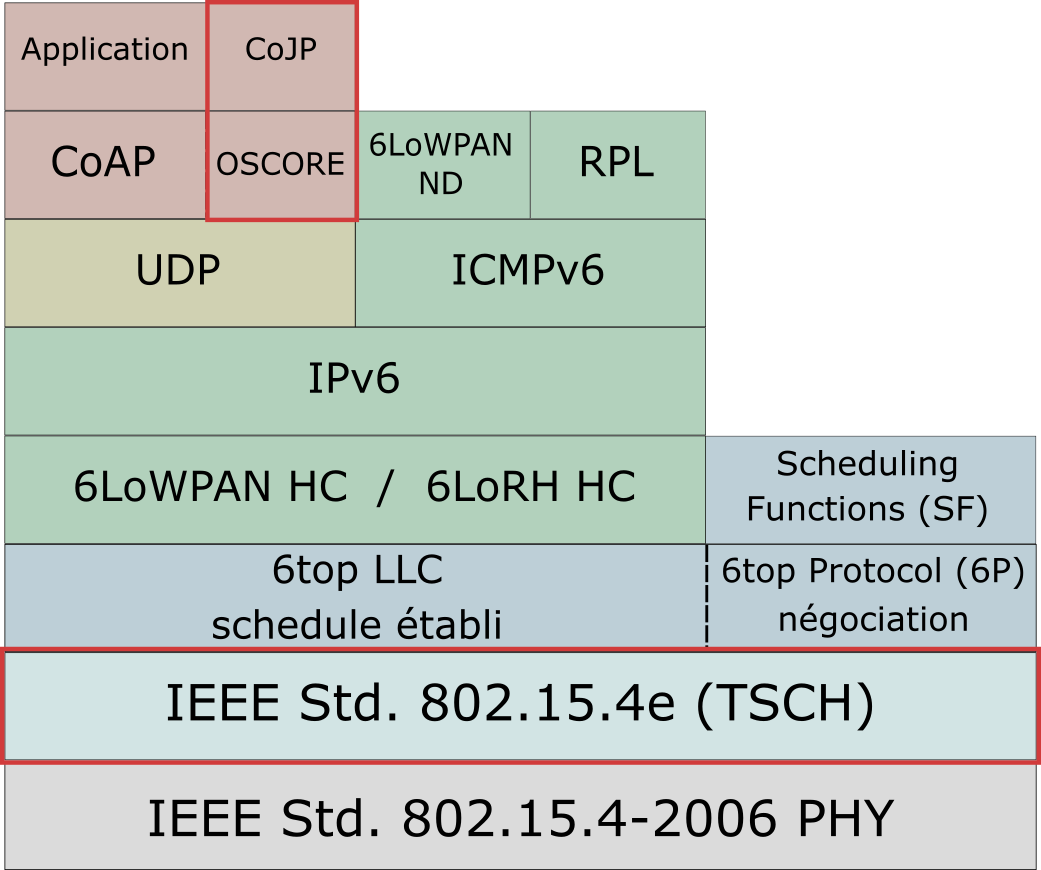
\includegraphics[width=0.6\linewidth]{6TiSCH_stack_focus}
    \caption{Pile réseau 6TiSCH}
    \end{figure}
    \end{overprint}
	}
	
    \subsection{Principes fondamentaux de TSCH}	
    
    \frame{
        \frametitle{Principes fondamentaux de TSCH}
        
        Combinaison de :
        \begin{enumerate}
        \item TDMA $\rightarrow$ multiplexage en temps       (\textit{timeslot})
        \item FDMA $\rightarrow$ multiplexage en fréquences  (\textit{channelOffset})
        \end{enumerate}
        \vspace{0.5cm}
        Une communication entre noeuds voisins est caractérisée par un couple (\textit{timeslot}, \textit{channelOffset}) où
        \begin{enumerate}
        \item \textit{timeslot} donne le moment de la communication
        \item \textit{channelOffset} donne la fréquence à laquelle elle a lieu
        \end{enumerate}
        
        \vspace{0.3cm}
        
        Les noeuds communiquant possèdent et partagent cette information\\
        $\rightarrow$ communications déterministes sur base d'un \textit{schedule}
        
    }
    
    \frame{
    
    \begin{center}
            \begin{columns}[onlytextwidth,T]

        \column{4cm}	
        \centering   
    \begin{figure}
    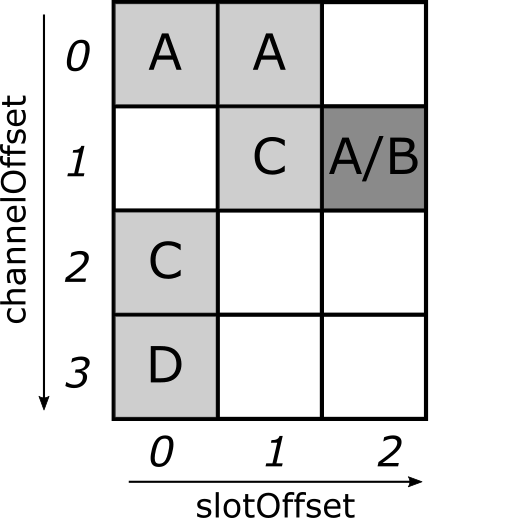
\includegraphics[width=4cm]{TSCH_basics_matrix}
    \caption{Matrice des communications}
    \end{figure}    	        
        \column{\dimexpr\linewidth-4cm}
    \begin{figure}
    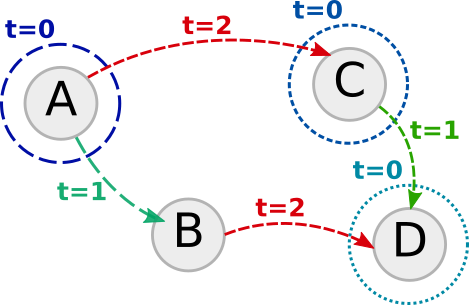
\includegraphics[width=5cm]{TSCH_basics_graph}
    \caption{Noeuds communiquant}
    \end{figure}    
	    \end{columns}
	\end{center}

    }

    \frame{
    \centering
    $f_{eff} = HoppSeq[f \:\: \text{mod} \:\: n_{ch}]\quad$ où $f = ASN + channelOffset$
    \vspace{0.1cm}
       \begin{figure}
    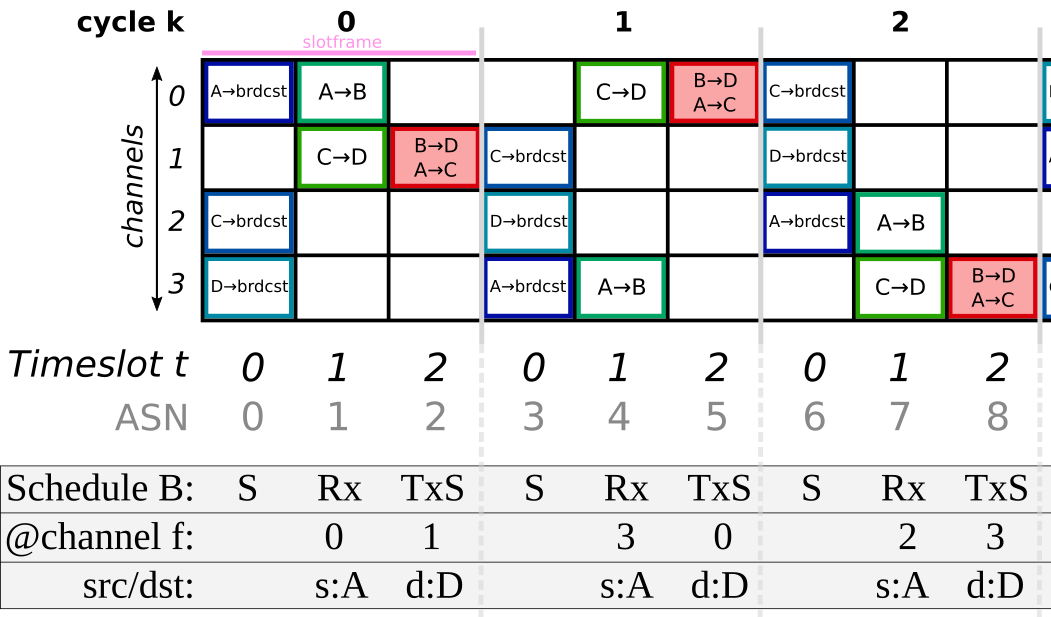
\includegraphics[width=0.8\linewidth]{TSCH_basics_schedule_croped}
    \caption{Effet de sauts de fréquence d'un cycle à l'autre de slotframe}
    \end{figure}
    }

    \subsection{La joining phase}
    
    \frame{
        \frametitle{La joining phase}
       
    
    }
    
    \section{Méthode NPEB et expérimentations}
    
    \frame{
		\frametitle{Outline}	% Sommaire
		\tableofcontents[currentsection]
		% options = pausesections; currentsection; hideallsubsections 
	}    
    
    \subsection{Principes de la méthode NPEB}
    
    \frame{
        \frametitle{Principes de la méthode NPEB}
    
    }
    
    
    \subsection{Évaluation de l'impact de sécurité sur la joining phase}	
	
    \frame{
        \frametitle{Impact de sécurité sur la joining phase}
    
    }
    
    \subsection{Évaluation des performances de la méthode NPEB}	

    \frame{
        \frametitle{Performances de la méthode NPEB}
    
    }
	
    \section{Conclusion}	
	
    \frame{
        \frametitle{Conclusion}
    
    }	
	
	\frame{
	\begin{center}
	    \Large{Performances des mécanismes de sécurité du framework 6TiSCH\\}
	    \vspace{0.3cm}
	    \Huge{Q\&A}
	\vspace{0.3cm}
	   \rule{11cm}{0.6pt}\\
	\end{center}
	}
	
\end{document}
